\chapter{Additional Background Information}
\label{app:cha:background}

This chapter  provides some additional background information  that may be
useful to fully understand particular design and implementation aspects.

\section{Public-key cryptography}
\label{app:sec:public-key-cryptography}

Public-key  cryptography describes  a form  of cryptography  where  a user
holds  two  different  keys,  a  \emph{private  key}  and  a  \emph{public
  key}.  These two  keys are  mathematically  related to  each other,  but
nobody can practically derive the private key from the public key.

The public key can be made  publicly available without any risk, while the
private key must  be kept very secret. A widely used  algorithm is the RSA
algorithm named  after its  creators \citet*{rivest77method}. It  has been
the first algorithm, that  was suitable for both encryption/decryption and
signing.  For more background information on public-key cryptosystems, you
are encouraged to read \cite{rivest77method,diffie76new}.

The RSA algorithm relies on the fact, that the factorization of reasonably
large numbers is  computationally very hard and no  efficient algorithm is
publicly known.  Especially  hard to factor are numbers  whose factors are
two randomly-chosen prime numbers of sufficient length.

In the following  I am going to describe  how the keys are set  up and how
they  are  used  to  encrypt/decrypt  or to  sign/validate  a  clear  text
message.  The provided  material  is  based on  the  information found  in
\cite{rivest77method} and \cite{diffie76new}.

According  to  \cite{rivest77method}   places  each  user  his  encryption
procedure $E$  in a publicly  accessible file (\eg database).   Using this
public file, any  other user is able to  retrieve the encryption procedure
of some other user (\ie the one he wants to send encrypted messages). Each
user keeps his decryption procedure $D$ secret.

The mentioned procedures $D$ and $E$ have the following properties:
\begin{enumerate}
\renewcommand{\theenumi}{\alph{enumi}}
\renewcommand{\labelenumi}{(\theenumi)}

\item Deciphering  the enciphered form of  a message $M$  yields $M$. That
  is,
  \begin{equation}
    \label{eq:1}
    D(E(M)) = M.
  \end{equation}
  \label{pubkey-cryptosystem-prop-1}
\item Both $D$ and $E$ are easy to compute.
  \label{pubkey-cryptosystem-prop-2}
\item The user does not reveal an  easy way to compute $D$ if he makes $E$
  publicly available.
  \label{pubkey-cryptosystem-prop-3}
\item  The enciphering  of a  previously ciphered  message $M$  results in
  $M$. That is,
  \begin{equation}
    \label{eq:2}
    E(D(M)) = M.
  \end{equation}
  \label{pubkey-cryptosystem-prop-4}
\end{enumerate}

A                  function                 $E$                 satisfying
(\ref{pubkey-cryptosystem-prop-1})--(\ref{pubkey-cryptosystem-prop-3})   is
said  to  be  a  \emph{``trap-door  one-way function''}  and  if  it  also
satisfies  (\ref{pubkey-cryptosystem-prop-4})  it  is a  \emph{``trap-door
  one-way permutation''} \cite{rivest77method,diffie76new}.

\subsection{Key setup}

The \emph{encryption  key} consists  of a pair  of positive  integers $(e,
n)$,  where $e$  is the  \emph{encryption exponent}  and $n$  is  used for
modulo  operations.  The \emph{decryption  key}  is  also  a pair  of  two
integers, where only the exponent differs, thus $(d, n)$ is the decryption
key and $d$  represents the \emph{decryption exponent}. $(e,  n)$ are made
publicly available.

\citet*{rivest77method} suggest the  following approach for the generation
of $(e, n)$ and  $(d, n)$. The fist step is to  compute $n$ as the product
of two very large, ``random'' primes $p$ and $q$:
\begin{equation*}
  \label{eq:compute-n}
n = p \cdot q.
\end{equation*}

Although you  publish $n$, nobody is  able to compute the  factors $p$ and
$q$ in  reasonably time due to  the enormous difficulty  of factoring $n$.
In \cite{rivest77method}  it is assumed,  that the computation of  $p$ and
$q$ from a given $n$ takes $1.5 \times 10^{29}$ operations, given that $n$
has a length  of $300$ digits. If one operation  took one microsecond, the
whole computation takes $4.9 \times 10^{15}$ years.

The  next step  is to  choose  $d$, therefore  one picks  a large,  random
integer that is \emph{co-prime}\footnote{two integers $a$ and $b$ are said
  to be co-prime  if they do not  have a common factor other  than $1$ and
  $-1$, \ie their greatest common divisor  (gcd) is $1$.} to $(p-1) \cdot
(q-1)$.\footnote{the term $(p-1)\cdot(q-1)$ is the result of \emph{Euler's
    Phi} or  \emph{Euler's totient function}  ($\phi$) applied to  $n$} In
other words, $d$ has to satisfy:
\begin{equation*}
  \label{eq:compute-d}
  gcd(d, (p-1) \cdot (q-1)) = 1.
\end{equation*}

Finally,  the integer $e$  is computed  from $p$,  $q$ and  $d$ to  be the
\emph{multiplicative inverse} of $d$, modulo $\phi(n)$:
\begin{equation*}
  \label{eq:compute-e}
  e \cdot d \equiv 1\ \ (mod\ (p-1) \cdot (q-1))
\end{equation*}

\subsection{Encryption and Decryption}

If  two  persons,  Alice  and   Bob,  want  to  send  each  other  private
(\ie encrypted)  messages,  they   both  retrieve  the  other's  publicly
available encryption  key first ---  Bob retrieves $(e_a, n_a)$  and Alice
retrieves $(e_b, n_b)$.

Let's say  Alice wants to send a  private message to Bob.   To encrypt the
message, she has to  represent it as an integer between $0$  and $n_b - 1$
(long  messages can  be broken  into smaller  blocks, so  that  each block
fulfills the requirement). Alice then  encrypts the message $M$ by raising
it to the $e_b$th power modulo $n_b$, the result is the cyphertext $C$:
\begin{equation*}
  \label{eq:encrypt-message}
  C \equiv E(M) \equiv M^{e_b}\ \ (mod\ \ n_b).
\end{equation*}

On reception  of the cyphertext  $C$, Bob raises  it to the  $d_b$th power
modulo $n_b$. He  is the only person, who knows $d_b$  and therefore he is
solely able to decrypt $C$:
\begin{equation*}
  \label{eq:decrypt-message}
  M \equiv D(C) \equiv C^{d_b}\ \ (mod\ \ n_b).
\end{equation*}

\subsection{Signing and Validating}

Electronic  signatures, \eg in electronic  mail systems,  especially when
used in  business transactions, must  provide provability to  the receiver
that  the message  originated from  the sender.   This is  more  than just
provide  mere \emph{authentication},  where the  recipient of  a digitally
signed message can  verify that the message came  from the sender. Digital
signatures must be  able to be used to convince  a ``judge'', that neither
the recipient did  forge the message, nor the sender  can deny sending the
message.

That means,  an electronic signature must  be \emph{message}-dependent, as
well as  \emph{signer}-dependent. If the  signature did not depend  on the
message itself, a dishonorable recipient  could just change the message or
attach the signature to a  completely different message before showing the
message/signature pair  to a judge. If  the signature would  not depend on
the \emph{signer}, obviously anybody could have signed the message.

\medskip

If   Bob  want  to   send  Alice   a  signed   message,  he   applies  his
\emph{decryption}  function $D_b$  to the  clear text  message  $M$, which
results in the signature $S$:

\begin{equation*}
  \label{eq:compute-signature}
  S = D_b(M).
\end{equation*}

To   perform  this,   the  cryptosystem   has  to   be   implemented  with
\emph{trap-door         one-way        permutations},        \ie property
(\ref{pubkey-cryptosystem-prop-4}) must hold.

This signature  can now  be encrypted using  Alice's public key  to ensure
privacy, there  is no need to  send the message along  with the signature,
since it can  be computed from it. On reception,  Alice first decrypts the
message which  results in the  plain signature $S$ again.   Applying Bob's
\emph{encryption} function to the  received signature (Alice knows who the
presumed sender  of the  message is) makes  perfect sense due  to property
(\ref{pubkey-cryptosystem-prop-4}):

\begin{equation*}
  \label{eq:validate-signature}
  M = E_b(S)
\end{equation*}

Bob cannot  later on deny that he  sent the message, since  nobody but him
could  have generated  the signature  $S$.  Alice  is able  to  convince a
``judge'', that  Bob did send the  message, since $E_b(S) =  M$. But Alice
cannot modify  $M$ or  provide a different  message $M'$ because  then she
would also need to compute $S' = D_b(M')$ as well.

\section{Calana}
\label{app:sec:calana}

\emph{Calana} is  a new Grid  scheduler approach proposed  by M.~Dalheimer
\cite{dalheimer05agentbased}.   The scheduler  uses  several \emph{agents}
and at  least one  \emph{broker}.

The  agents are  responsible for  single resource.   That means  they know
whether the resource is free or  not. They are also capable to acquire new
or cancel previously made reservations on this resource.

If  a user  wants to  submit a  job to  the grid  environment,  the broker
initiates an  \emph{auction} among the  connected agents. The job  is then
assigned to the resource that belongs to the agent that won the auction.

\subsection{Architecture}

An  abstract   view  over   the  architecture  of   Calana  is   shown  in
Figure~\ref{fig:calana-architecture}.   For a  detailed discussion  of the
protocol  that  is   used  to  perform  the  auctions,   have  a  look  at
\cite{dalheimer06calanaprotocol} and \cite{petry06}.

\begin{figure}[ht]
  \centering
  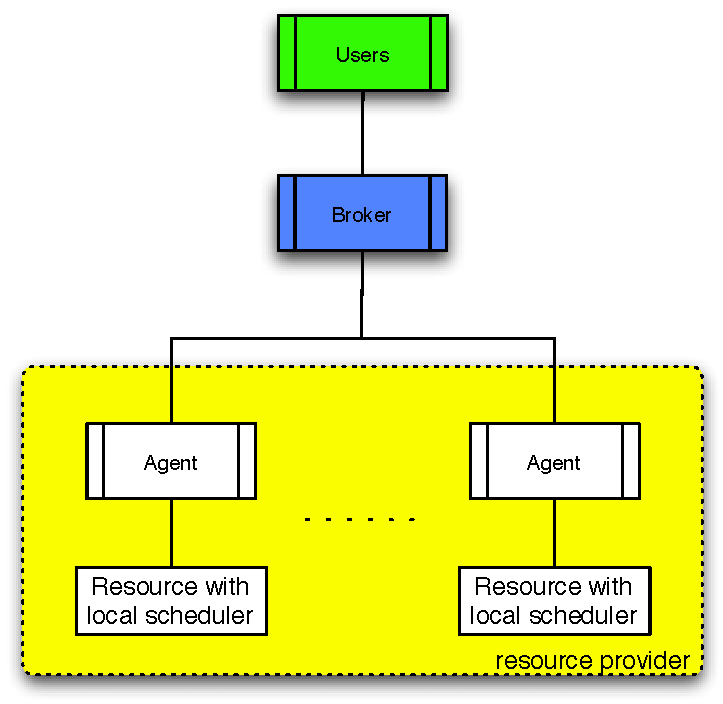
\includegraphics[scale=0.5]{calana-architecture}
  \caption{Architecture of Calana}
  \label{fig:calana-architecture}
\end{figure}

The main steps of such an auction are can be described as follows:

\begin{enumerate}
\item When a user submits a job to the Calana-broker, the broker will open
  up an auction and try to \emph{book} a resource for the task.
\item    For   each   task    an   auction    is   created    by   sending
  \texttt{BookingReq}-messages to the connected agents.
\item The agents will make  one or more \emph{reservations} on their local
  scheduler  and  answer with  a  \texttt{AuctionBid}.   Bids contain  for
  example  the  cost  of   using  the  resource  and  various  reservation
  parameters  such  as  the   earliest  start-time  and  duration  of  the
  reservation.
\item To make a decision, the  broker judges all received bids and chooses
  the     best     one      according     to     some     preference-model
  \cite{dalheimer05agentbased, petry06}.
\item If  the user  accepts the decision,  the broker  \emph{confirms} the
  reservation.
\end{enumerate}

\subsection{Job-state model}
\label{app:sec:calana-job-model}

To reflect the possibility  to \emph{make}, \emph{confirm}, \emph{use} and
\emph{cancel} reservations on some resource, the job-state model had to be
extended. We discussed about a common state-model for the jobs and came to
the  consensus of  adopting  the  \gls{glo:BES} model  to  our needs  (see
Figure~\ref{fig:bes-calana-job-model}).

\begin{figure}[h]
  \centering
  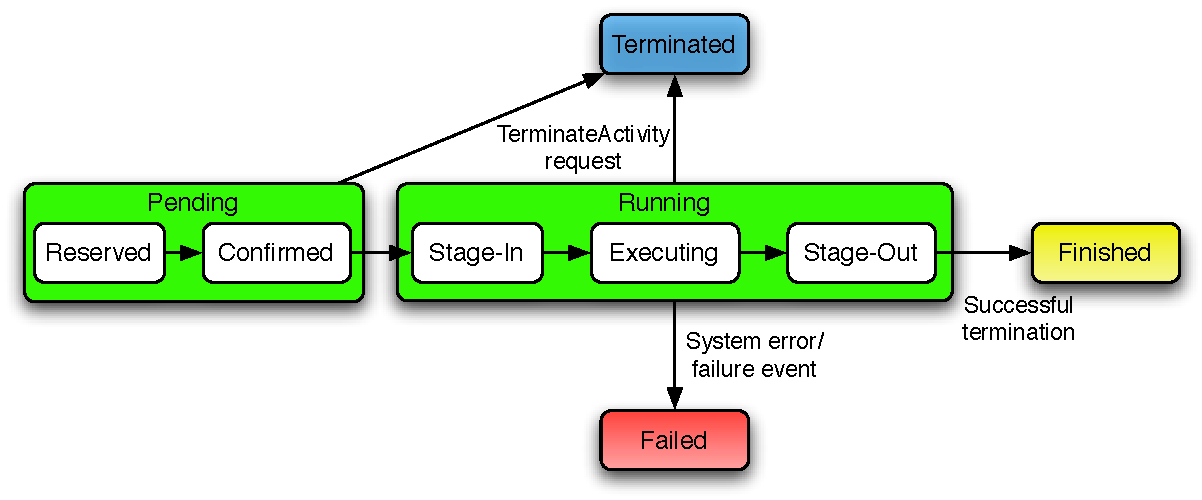
\includegraphics[scale=.55]{bes-calana-job-model}
  \caption[Calana Job Model]{The common job model proposed by the Calana
    Grid scheduler.}
  \label{fig:bes-calana-job-model}
\end{figure}

%%% Local Variables: 
%%% mode: latex
%%% TeX-master: "main.tex"
%%% End: 
